\chapter{Categorical Transformations}\label{ch:cattransformation}
\markright{Ch. \ref{ch:cattransformation}: Categorical Transformations}

\section{Conversion, Obversion, and Contraposition}\label{sec:conv_obv_cont}

Now that we have shown the wide range of statements that can be represented in our four standard logical forms A, E, I, and O, it is time to begin constructing arguments with them. The arguments we are going to look at are sometimes called ``immediate inferences'' because they only have one premise. We are going to learn to identify some valid forms of these one-premise arguments by looking at ways you can transform so that a true sentence will stay true and a false sentence will stay false. Remember that on page \pageref{def:truth_value} we said that the \gls{truth value} of a sentence is simply whether the sentence is true or false. So we can say that the transformations we will be looking at here preserve the truth values of the sentences.

Consider the statements, ``No dogs are reptiles'' and ``No reptiles are dogs.'' They have the same truth value and basically mean the same thing. On the other hand if you change ``All dogs are mammals'' into ``All mammals are dogs'' you turn a true sentence into a false one. In this section we are going to look at three ways of transforming categorical statements---conversion, obversion, and contraposition---and use Venn diagrams to determine whether these transformations also lead to a change in truth value. From there we can identify valid argument forms.

\section{Conversion}\label{sec:conversion}

The two examples in the last paragraph are examples of conversion. \textsc{\gls{conversion}} \label{def:conversion} is the process of transforming a categorical statement by switching the subject and the predicate. When you convert a statement, it keeps its form---an A statement remains an A statement, an E statement remains an E statement---however it might change its truth value.  The Venn diagrams in Figure \ref{fig:conversion} illustrate this.

\begin{figure}[!ht]
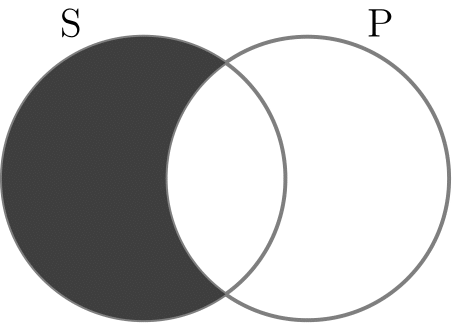
\includegraphics[width=0.4\textwidth]{2venn2}
\begin{minipage}[c]{0.1\textwidth}\vspace{-2.5cm}\hspace{.4cm}$\to$\end{minipage}
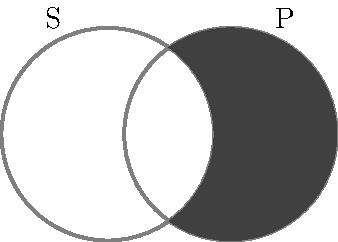
\includegraphics[width=0.4\textwidth]{2venn3}


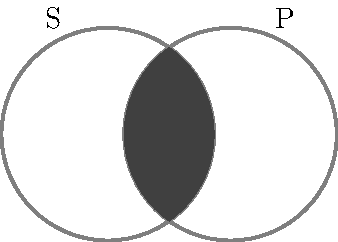
\includegraphics[width=0.4\textwidth]{2venn4}
\begin{minipage}[c]{0.1\textwidth}\vspace{-2.5cm}\hspace{.4cm}$\to$\end{minipage}
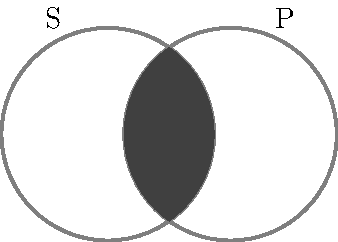
\includegraphics[width=0.4\textwidth]{2venn4}


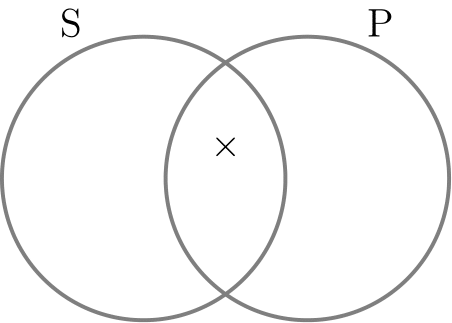
\includegraphics[width=0.4\textwidth]{2venn5}
\begin{minipage}[c]{0.1\textwidth}\vspace{-2.5cm}\hspace{.4cm}$\to$\end{minipage}
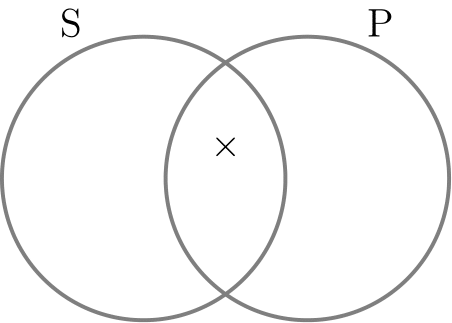
\includegraphics[width=0.4\textwidth]{2venn5}


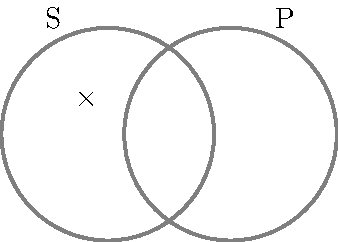
\includegraphics[width=0.4\textwidth]{2venn6}
\begin{minipage}[c]{0.1\textwidth}\vspace{-2.5cm}\hspace{.4cm}$\to$\end{minipage}
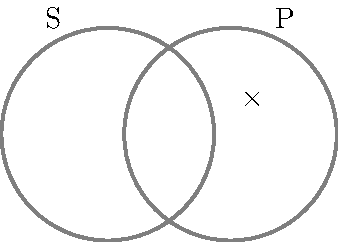
\includegraphics[width=0.4\textwidth]{2venn7}
\caption{Conversions of all quantified categorical sentences.}
\label{fig:conversion}
\end{figure}

As you can see, the Venn diagram for the converse of an E statement is exactly the same as the original E statement, and likewise for I statements. This means that the two statements are logically equivalent. Recall that two statements are logically equivalent if they always have the same truth value. (See page \ref{def:logical_equivalence}). In this case, that means that if an E statement is true, then its converse is also true, and if an E statement is false, then its converse is also false. For instance, ``No dogs are reptiles'' is true, and so is ``No reptiles are dogs.'' On the other hand ``No dogs are mammals'' is false, and so is ``No mammals are dogs.''

Likewise, if an I statement is true, its converse is true, and if an I statement is false, than its converse is false. ``Some dogs are pets'' is true, and so is ``Some pets are dogs.'' On the other hand ``Some dogs can fly'' is false and so is ``Some flying things are dogs.''

The converses of A and O statements are not so illuminating. As you can see from the Venn diagrams, these statements are not identical to their converses. They also don't contradict their converses. If we know that an A or O statement is true, we still don't know anything about their converses. We say their truth value is undetermined.

Because E and I statements are logically equivalent to their converses, we can use them to construct valid arguments. Recall from Chapter 2 (page \pageref{def:valid}) that an argument is valid if it is impossible for its conclusion to be false whenever its premises are true. Because E and I are logically equivalent to their converses, the two argument forms in Figure \ref{fig:conversion_arguments} are valid.


\begin{kormanize}
\premise{No $S$ are $P$.}
\conclusion{No $P$ are $S$.}
\end{kormanize}


\begin{kormanize}
\premise{Some $S$ are $P$.}
\conclusion{Some $P$ are $S$.}
\end{kormanize}

Notice that these are argument forms, with variables in the place of the key terms. This means that these arguments will be valid no matter what; $S$ and $P$ could be people, or squirrels, or the Gross Domestic Product of industrialized nations, or anything, and the arguments are still valid. While these particular argument forms may seem trivial and obvious, we are beginning to see some of the power of formal logic here. We have uncovered a very general truth about the nature of validity with these two argument forms.

The truth value of the converses of A and O statements, on the other hand, are undetermined by the truth value of the original statements. This means we cannot construct valid arguments from them. Imagine you have an argument with an A or O statement as its premise and the converse of that statement as the conclusion. Even if the premise is true, we know nothing about the truth of the conclusion. So there are no valid argument forms to be found here.

\section{Obversion}\label{sec:obversion}


Obversion is a more complex process. To understand what an obverse is, we first need to define the complement of a class. The \textsc{\gls{complement}} \label{def:complement} of a class is everything that is not in the class. So the complement of the class of dogs is everything that is not a dog, including not just cats, but battleships, pop songs, and black holes. In English we can easily create a name for the complement of any class using the prefix ``non-''. So the complement of the class of dogs is the class of non-dogs. We will use complements in defining both obversion and contraposition.


The \textsc{\gls{obversion}} \label{def:obversion} of a categorical proposition is a new proposition created by changing the quality of the original proposition and switching its predicate to its complement. Obversion is thus a two step process. Take, again, the proposition ``All dogs are mammals.'' For step 1, we change its quality, in this case going from affirmative to negative. That gives us ``No dogs are mammals.'' For step 2, we take the complement of the predicate. The predicate in this case is ``mammals'' so the complement is ``non-mammals.'' That gives us the obverse ``No dogs are non-mammals.''

We can map this process out using Venn diagrams. Let's start with an A statement and change the quality, which turns it into an E statement.

\begin{figure}[!ht]
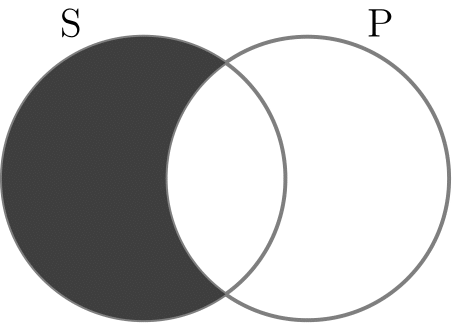
\includegraphics[width=0.4\textwidth]{2venn2}
\begin{minipage}[c]{0.1\textwidth}\vspace{-2.5cm}\hspace{.4cm}$\to$\end{minipage}
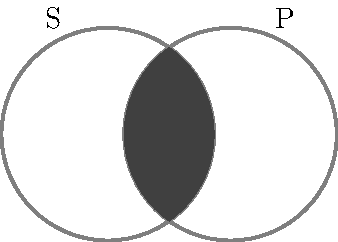
\includegraphics[width=0.4\textwidth]{2venn4}
\caption{Changing the quality of mood A into mood E.}
\label{fig:obversion_step1}
\end{figure}

Now what happens when we take the complement of $P$? That means we will shade in all the parts of S that are non-$P$, which puts us back where we started. We still have an E statement, but it is now equivalent to the A statement.

\begin{figure}[!ht]
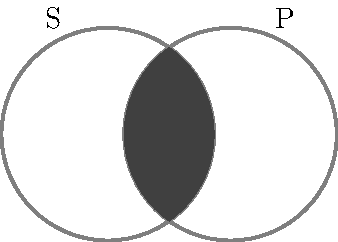
\includegraphics[width=0.4\textwidth]{2venn4}
\begin{minipage}[c]{0.1\textwidth}\vspace{-2.5cm}\hspace{.4cm}$\to$\end{minipage}
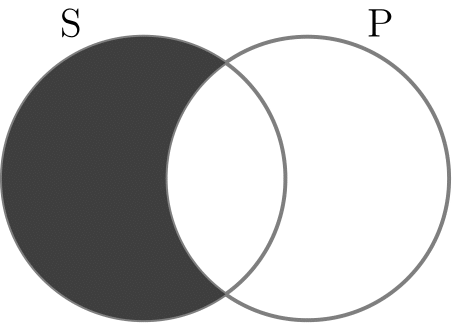
\includegraphics[width=0.4\textwidth]{2venn2}
\caption{Complement of mood E is equivalent to mood A.}
\label{fig:obversion_step2}
\end{figure}

The final statement is logically equivalent to the original A statement. It has the same form as an E statement, but because we have changed the predicate, it is not logically equivalent to an A statement. As you can see from Figure \ref{fig:obversion} this is true for all four forms of categorical statement.


This in turn gives us four valid argument forms, which are shown in figure~\ref{fig:obversion_arguments}

\begin{figure}
\begin{minipage}[t]{0.4\textwidth}
\begin{kormanize}
\premise{All $S$ are $P$.}
\conclusion{No $S$ are non-$P$.}
\end{kormanize}
\end{minipage}\hspace{1cm}
\begin{minipage}[t]{0.4\textwidth}
\begin{kormanize}
\premise{No $S$ is $P$.}
\conclusion{All $S$ are non-$P$.}
\end{kormanize}
\end{minipage}

\vspace{1cm}

\begin{minipage}[t]{0.4\textwidth}
\begin{kormanize}
\premise{Some $S$ is $P$.}
\conclusion{Some $S$ is not non-$P$.}
\end{kormanize}
\end{minipage}\hspace{1cm}
\begin{minipage}[t]{0.4\textwidth}
\begin{kormanize}
\premise{Some $S$ is non-$P$.}
\conclusion{Some $S$ is not $P$.}
\end{kormanize}
\end{minipage}
\caption{Four valid arguments from obversion.}
\label{fig:obversion_arguments}
\end{figure}

One further note on complements. We don't just use complements to describe sentences that come out of obversion and contraposition. We can also perform these operations on statements that already have complements in them. Consider the sentence ``Some $S$ are non-$P$.'' Its Venn diagram is in figure~\ref{fig:moodo_example}

\begin{marginfigure}
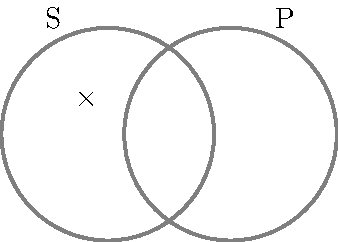
\includegraphics{2venn6}
\caption{Example of a mood O sentence.}
\label{fig:moodo_example}
\end{marginfigure}


How would we take the obverse of this statement? Step 1 is to change the quality, making it ``Some $S$ are not non-$P$.'' Now how do we take the complement of the predicate? We could write ``non-non-$P$,'' but if we think about it for a second, we'd realize that this is the same thing as $P$. So we can just write ``Some $S$ is not $P$.'' This is logically equivalent to the original statement, which is what we wanted.

Taking the converse of ``Some $S$ are non-$P$'' also takes a moment of thought. We are supposed to reverse subject and predicate. But does that mean that the ``non-'' moves to the subject position along with the ``$P$''? Or does the ``non-'' now attach to the $S$? We saw that E and I statements kept their truth value after conversion, and we want this to still be true when the statements start out referring to the complement of some class. This means that the ``non-'' has to travel with the predicate, because ``Some $S$ are non-$P$'' will always have the same truth value as ``Some non-$P$ are $S$.'' Another way of thinking about this is that the ``non-'' is part of the name of the class that forms the predicate of ``Some $S$ are non-$P$.'' The statement is making a claim about a class, and that class happens to be defined as the complement of another class. So, the bottom line is when you take the converse of a statement where one of the terms is a complement, move the ``non-'' with that term.

\section{Contraposition}\label{sec:contraposition}

\textsc{\Gls{contraposition}} is a two-step process, like obversion, but it doesn't always lead to results that are logically equivalent to the original sentence. The contrapositive of a categorical sentence is the sentence that results from reversing subject and predicate and then replacing them with their complements. Thus ``All $S$ are $P$'' becomes ``All non-$P$ are non-$S$.''

Figure \ref{fig:contraposition} shows the corresponding Venn diagrams. Like conversion, applying contraposition to two of the forms gives us statements that are logically equivalent to the original. This time, though, it is forms A and O that come through the process without changing their truth value.


\begin{figure}[!ht]
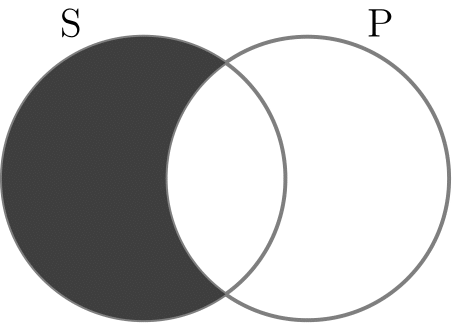
\includegraphics[width=0.4\textwidth]{2venn2}
\begin{minipage}[c]{0.1\textwidth}\vspace{-2.5cm}\hspace{.4cm}$\to$\end{minipage}
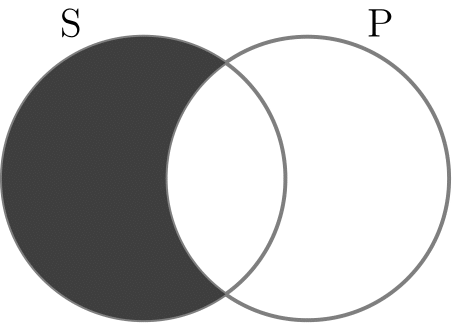
\includegraphics[width=0.4\textwidth]{2venn2}

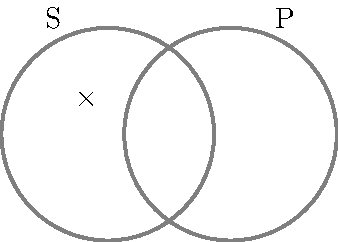
\includegraphics[width=0.4\textwidth]{2venn6}
\begin{minipage}[c]{0.1\textwidth}\vspace{-2.5cm}\hspace{.4cm}$\to$\end{minipage}
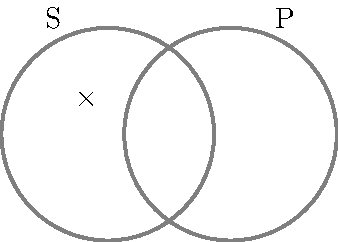
\includegraphics[width=0.4\textwidth]{2venn6}
\caption{Contrapositions of all quantified categorical sentences.}
\label{fig:contraposition}
\end{figure}


This then gives us two valid argument forms, shown in Figure \ref{fig:contraposition_arguments}. If you have an argument with an A or O statement as its premise and the contraposition of that statement as the conclusion, you know it must be valid. Whenever the premise is true, the conclusion must be true, because the two statements are logically equivalent. On the other hand, if you had an E or an I statement as the premise, the truth of the conclusion is undetermined, so these arguments would not be valid.

\begin{figure}
\begin{minipage}[t]{0.4\textwidth}
\begin{kormanize}
\premise{All $S$ is $P$.}
\conclusion{All non-$P$ are non-$S$.}
\end{kormanize}
\end{minipage}\hspace{1cm}
\begin{minipage}[t]{0.4\textwidth}
\begin{kormanize}
\premise{Some $S$ is non-$P$.}
\conclusion{Some non-$P$ is not non-$S$.}
\end{kormanize}
\end{minipage}
\caption{Two valid arguments from contraposition.}
\label{fig:contraposition_arguments}
\end{figure}

\section{Evaluating Short Arguments}\label{sec:ESA}

So far we have seen eight valid forms of argument with one premise: two arguments that are valid by conversion, four that are valid by obversion, and two that are valid by contraposition. As we said, short arguments like these are sometimes called ``immediate inferences,'' because your brain just flits automatically from the truth of the premises to the truth of the conclusion. Now that we have identified these valid forms of inference, we can use this knowledge to see whether some of the arguments we encounter in ordinary language are valid. We can now tell in a few cases if our brain is right to flit so seamlessly from the premise to the conclusion.

In the real world, the inferences we make are messy and hard to classify. Much of the complexity of this issue is tackled in the parts of the complete version of this text that cover critical thinking. Part \ref{part:critical_thinking} of this text, on critical thinking. Right now we are just going to deal with a limited subset of inferences: immediate inferences that might be based on conversion, obversion, or contraposition. Let's start start with the uncontroversial premise ``All dogs are mammals.'' Can we infer from this that all non-mammals are non-dogs? In canonical form, the argument would look like this.

\begin{kormanize}
\premise{ All dogs are mammals.}
\conclusion{ All non-mammals are non-dogs.}
\end{kormanize}

Evaluating an immediate inference like this is a four step process. First, identify the subject and predicate classes. Second, draw the Venn diagram for the premise. Third, see if the Venn diagram shows that the conclusion must be true. If it must be, then the argument is valid. Finally, if the argument is valid, identify the process that makes it valid. (You can skip this step if the argument is invalid.)

The Venn diagram for the premise shades out the possibility that there are dogs that aren't mammals. For step three, we ask, does this mean the conclusion must be true?  In this case, it does. The same shading implies that everything that is not a mammal must also not be a dog. In fact, the Venn diagram for the premise and the Venn diagram for the conclusion are the same. So the argument is valid. This means that we must go on to step four and identify the process that makes it valid. In this case, the conclusion is created by reversing subject and predicate and taking their complements, which means that this is a valid argument by contraposition.

Now, remember what it means for an argument to be valid. \label{valid_definition_reinforcement} As we said on page \pageref{def:valid}, an argument is valid if it is impossible for the premises to be true and the conclusion false. This means that we can have a valid argument with false premises, so long as it is the case that \emph{if} the premises were true, the conclusion would have to be true. So if the argument above is valid, then so is this one:

\begin{kormanize}
\premise{ All dogs are reptiles.}
\conclusion{All non-reptiles are non-dogs.}
\end{kormanize}

The premise is now false: all dogs are not reptiles. However, \emph{if} all dogs were reptiles, then it would also have to be true that all non-reptiles are non-dogs. The Venn diagram works the same way.



The Venn diagram for the premise still matches the Venn diagram for the conclusion. Only the labels have changed. The fact that this argument form remains true even with a false premise is just a variation on a theme we saw in
Figure \ref{fig:valid_sound} when we saw a valid argument (with false premises) for the conclusion ``Socrates is a carrot.'' So arguments by transposition, just like any argument, can be valid even if they have false premises. The same is true for arguments by conversion and obversion.

Arguments like these can also be invalid, even if they have true premises and a true conclusion. Remember that A statements are not logically equivalent to their converse. So this is an invalid argument with a true premise and a false conclusion:

\begin{kormanize}
\premise{ All dogs are mammals.}
\conclusion{All mammals are dogs.}
\end{kormanize}

This is an argument by conversion on an mood-A statement, which is invalid. The argument remains invalid, even if we substitute in a predicate where the conclusion happens to be true. For instance this argument is invalid.

\begin{kormanize}
\premise{  All dogs are \textit{Canis familiaris}.}
\conclusion{ All \textit{Canis familiaris} are dogs.}
\end{kormanize}

The Venn diagrams for the premise and conclusion of this argument will be just like the ones for the previous argument, just with different labels. So even though the argument has a true premise and a true conclusion, it is still invalid, because it is possible for an argument of this form to have a true premise and a false conclusion. This is an unreliable argument form that just happened, in this instance, not to lead to a false conclusion. This again is just a variation on a theme we saw in Chapter \ref{ch:basicevaluation}, in Figure \ref{arg:invalid_paris}, when we saw an invalid argument for the conclusion that Paris was in France.
